\section{聚类分析}

\subsection{聚类性能度量}
首先是下面会用到的几个量:
\begin{equation}
    \begin{aligned}
        \mu_i &= \dfrac 1{|C|}\sum\limits_{1 \leq i \leq |C|} \boldsymbol{x}_i \\
        \operatorname{avg}(C) &= \dfrac{2}{|C|(|C|-1)} \sum\limits_{1 \leq i < j \leq |C|} \operatorname{dist}(\boldsymbol{x}_i, \boldsymbol{x}_j) \\
        \operatorname{diam}(C) &= \max_{1 \leq i < j \leq |C|} \operatorname{dist}(\boldsymbol{x}_i, \boldsymbol{x}_j) \\
        d_{\min}(C_i, C_j) &= \min_{\boldsymbol{x}_i \in C_i, \boldsymbol{x}_j \in C_j} \operatorname{dist}(\boldsymbol{x}_i, \boldsymbol{x}_j) \\
        d_{\text{cen}}(C_i, C_j) &= \operatorname{dist}(\mu_i, \mu_j)
        \end{aligned}
\end{equation}

其中,$\operatorname{avg}(C)$ 表示簇 $C$ 内样本间的平均距离,$\operatorname{diam}(C)$ 表示簇 $C$ 内样本间的最远距离,
$d_{\min}(C_i, C_j)$ 表示簇 $C_i$ 和 $C_j$ 最近样本间的距离,$d_{\text{cen}}(C_i, C_j)$ 表示簇 $C_i$ 和 $C_j$ 中心点间的距离,
$\mu_i$ 表示簇 $C$ 的中心点。

\begin{itemize}
    \item DB 指数:
    \begin{equation}
        \operatorname{DBI} = \dfrac 1k \sum\limits_{i=1}^k{\max_{j \neq i}\left(\dfrac{\operatorname{avg}(C_i)
         + \operatorname{avg}(C_j)}{d_{\text{cen}}(\mu_i, \mu_j)}\right)}
    \end{equation}\par
    DB 指数越小,聚类效果越好。
    \item Dunn 指数:
    \begin{equation}
        \operatorname{DI} = \min_{1 \leq i \leq k}\left\{\min_{j \neq i}\left(\dfrac{d_{\min}(C_i, C_j)}
        {\max\limits_{1 \leq l \leq k}\operatorname{diam}(C_l)}\right)\right\} 
        = \dfrac{\min_{1 \leq k < k' \leq m}d_{\min}(C_k, C_{k'})}{\max_{1 \leq l' \leq m}\operatorname{diam}(C_{l'})}
    \end{equation}\par
    Dunn 指数越大,聚类效果越好。
\end{itemize}

在衡量两个样本$\boldsymbol{x}_i = \left(x_{i1};x_{i2};\dots;x_{in}\right)$ 
和 $\boldsymbol{x}_j = \left(x_{j1};x_{j2};\dots;x_{jn}\right)$ 的距离时,常用的是“闵可夫斯基距离”:
\begin{equation}
    \operatorname{dist}_{\text{mk}}(\boldsymbol{x}_i, \boldsymbol{x}_j)
     = \left(\sum\limits_{u = 1}^n{|x_{iu} - x_{ju}|^p}\right)^{\frac 1p}
\end{equation}

上式即为 $\boldsymbol{x}_i - \boldsymbol{x}_j$ 的 $\boldsymbol{L}_p$ 范数 $\|\boldsymbol{x}_i - \boldsymbol{x}_j\|_p$。
当 $p = 1$ 时,称为“曼哈顿距离”;当 $p = 2$ 时,称为“欧式距离”。

\subsection{原型聚类 - Kmeans 算法}
此类算法假设聚类结构能通过一组原型刻画,在现实聚类任务中极为常用。
通常情况下,算法先对原型进行初始化,再对原型进行迭代更新求解。

Kmeans 算法针对聚类所得的簇划分 $\mathcal{C} = \left\{C_1, C_2, \dots, C_k\right\}$ 最小化均方误差
\begin{equation}
    E = \sum\limits_{i=1}^k{\sum\limits_{\boldsymbol{x} \in C_i} ||\boldsymbol{x} - \mu_i||_2^2}
\end{equation}

其中 $\mu_i = \frac 1{|C_i|}\sum_{\boldsymbol{x} \in C_i} \boldsymbol{x}$ 是簇 $C_i$ 的均值向量,即“原型”。
$E$ 值在一定程度上刻画了簇内样本围绕簇均值向量的紧密程度,$E$ 值越小,则簇内样本相似度越高。

\begin{algorithm}[H]
    \renewcommand{\algorithmicrequire}{\textbf{Input:}}
	\renewcommand{\algorithmicensure}{\textbf{Output:}}
    \caption{$k$-Means 算法}
    \begin{algorithmic}[1]
        \REQUIRE 样本集 $D = \left\{\boldsymbol{x}_1, \boldsymbol{x}_2, \cdots, \boldsymbol{x}_m\right\}$,聚类簇数 $k$
        \ENSURE 簇划分 $\mathcal C = \left\{C_1, C_2, \dots, C_k\right\}$
        \STATE 从 $D$ 中随机选择 $k$ 个样本作为初始均值向量 $\left\{\boldsymbol{\mu}_1, \boldsymbol{\mu}_2, \cdots, \boldsymbol{\mu}_k\right\}$
        \WHILE{当前均值向量被更新且不是第一次进入循环}
        \STATE 令 $C_i = \varnothing(1 \leq i \leq k)$
        \FOR{$j = 1, 2, \cdots, m$}
            \STATE 计算样本 $\boldsymbol{x}_j$ 与各均值向量 $\boldsymbol{\mu}_i(1 \leq i \leq k)$ 的距离:
            $d_{ji} = \|\boldsymbol{x}_j - \boldsymbol{\mu}_i\|_2$
            \STATE 根据距离最近的均值向量确定 $\boldsymbol{x}_j$ 的簇标记:
            $\lambda_j = \arg\min_{i \in \left\{1, 2, \cdots, k\right\}}d_{ji}$
            \STATE 将样本 $\boldsymbol{x}_j$ 划入对应的簇: 
            $C_{\lambda_j} = C_{\lambda_j} \bigcup \left\{\boldsymbol{x}_j\right\}$
        \ENDFOR
        \FOR{$i = 1, 2, \cdots, k$}
            \STATE 计算新的均值向量 
            $\boldsymbol{\mu}_i' = \frac 1{|C_i|}\sum_{\boldsymbol{x} \in C_i} \boldsymbol{x}$
            \IF{$\boldsymbol{\mu}_i' \neq \boldsymbol{\mu}_i$}
                \STATE 将当前均值向量 $\boldsymbol{\mu}_i$ 更新为 $\boldsymbol{\mu}_i'$
            \ELSE
                \STATE 保持当前均值向量不变
            \ENDIF
        \ENDFOR
        \ENDWHILE
    \end{algorithmic}
\end{algorithm}

\subsection{密度聚类 - DBSCAN 算法}
此类算法假设聚类结构能通过样本分布的紧密程度来确定。
通常情况下,密度聚类算法从样本密度的角度来考察样本之间的可连接性,并基于可连接样本不断扩展聚类簇来获得最终的聚类结果。

DBSCAN 算法是一种著名的密度聚类算法,它基于一组“邻域”参数 $(\epsilon, MinPts)$ 来刻画样本分布的紧密程度。
给定数据集 $D = \left\{\boldsymbol{x}_1, \boldsymbol{x}_2, \dots, \boldsymbol{x}_m\right\}$,定义下面几个概念:
\begin{itemize}
    \item $\epsilon$-邻域:对 $\boldsymbol{x}_j \in D$,其 $\epsilon$-邻域包含样本集 $D$ 中与 $\boldsymbol{x}_j$ 的距离不大于 $\epsilon$ 的样本,
    即 $N_{\epsilon}\left(\boldsymbol{x}_{j}\right)=\left\{\boldsymbol{x}_{i} \in D \mid \operatorname{dist}\left(\boldsymbol{x}_{i}, \boldsymbol{x}_{j}\right) \leqslant \epsilon\right\}$;
    \item 核心对象:若 $\boldsymbol{x}_j$ 的 $\epsilon$-邻域至少包含 $MinPts$ 个样本,
    即 $\left|N_\epsilon(\boldsymbol{x}_j)\right| \geq MinPts$,则 $\boldsymbol{x}_j$ 是一个核心对象;
    \item 密度直达:若 $\boldsymbol{x}_j$ 在 $\boldsymbol{x}_i$ 的 $\epsilon$-邻域中,
    且 $\boldsymbol{x}_i$ 是核心对象,则称 $\boldsymbol{x}_j$ 由 $\boldsymbol{x}_i$ 密度直达;
    \item 密度可达:对 $\boldsymbol{x}_i$ 与 $\boldsymbol{x}_j$,若存在样本序列 $\boldsymbol{p}_1, \boldsymbol{p}_2, \dots, \boldsymbol{p}_n$,其中 $\boldsymbol{p}_1 = \boldsymbol{x}_i$,$\boldsymbol{p}_n = \boldsymbol{x}_j$ 
    且 $\boldsymbol{p}_{i+1}$ 由 $\boldsymbol{p}_i$ 密度直达,则称 $\boldsymbol{x}_j$ 由 $\boldsymbol{x}_i$ 密度可达;
    \item 密度相连:对 $\boldsymbol{x}_i$ 和 $\boldsymbol{x}_j$,若存在 $\boldsymbol{x}_k$ 使得 $\boldsymbol{x}_i$ 
    与 $\boldsymbol{x}_j$ 均由 $\boldsymbol{x}_k$ 密度可达,则称 $\boldsymbol{x}_i$ 与 $\boldsymbol{x}_j$ 密度相连。
\end{itemize}

\begin{figure}[htbp]
    \centering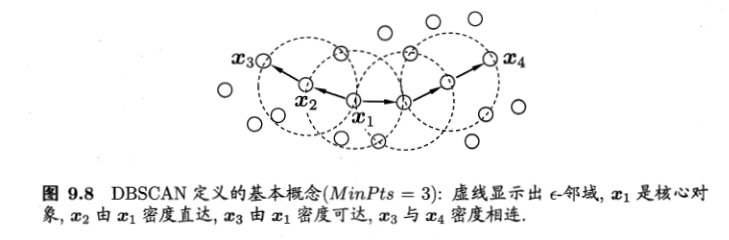
\includegraphics[scale = 0.5]{DBSCAN.png}
\end{figure}

DBSCAN 将“簇”定义为:有密度可达关系导出的最大的密度相连样本集合。

形式化地,给定邻域参数 $(\epsilon, MinPts)$,簇 $C \subseteq D$ 是满足以下性质的非空样本子集:
\begin{itemize}
    \item 连接性:$\boldsymbol{x}_i \in C$,
    $\boldsymbol{x}_j \in C \Longrightarrow$ $\boldsymbol{x}_i$ 和 $\boldsymbol{x}_j$ 密度相连
    \item 最大性:$\boldsymbol{x}_i \in C$,$\boldsymbol{x}_j$ 
    由 $\boldsymbol{x}_i$ 密度可达 $\Longrightarrow$ $\boldsymbol{x}_j \in C$

\end{itemize}

实际上,若 $\boldsymbol{x}$ 为核心对象,则 $\boldsymbol{x}$ 密度可达的所有样本的集合记为 
\begin{equation}
    X = \left\{\boldsymbol{x}' \in D \mid \boldsymbol{x}' \text{由}\boldsymbol{x}\text{密度可达}\right\}
\end{equation}
则 $X$ 即为满足连接性和最大性的簇。

\begin{algorithm}[H]
    \renewcommand{\algorithmicrequire}{\textbf{Input:}}
	\renewcommand{\algorithmicensure}{\textbf{Output:}}
    \caption{DBSCAN 算法}
    \begin{algorithmic}[1]
        \REQUIRE 样本集 $D = \left\{\boldsymbol{x}_1, \boldsymbol{x}_2, \cdots, \boldsymbol{x}_m\right\}$,邻域参数 $(\epsilon, MinPts)$
        \ENSURE 簇划分 $C = \left\{C_1, C_2, \cdots, C_k\right\}$
        \STATE 初始化核心对象集合:$\Omega = \varnothing$
        \FOR{$j = 1, 2, \cdots, m$}
            \STATE 确定 $\boldsymbol{x}_j$ 的 $\epsilon$-邻域 $N_\epsilon(\boldsymbol{x}_j)$
            \IF{$|N_\epsilon(\boldsymbol{x}_j)| \geq MinPts$}
                \STATE 将 $\boldsymbol{x}_j$ 加入核心对象集合:$\Omega = \Omega \bigcup \left\{\boldsymbol{x}_j\right\}$
            \ENDIF
        \ENDFOR
        \STATE 初始化聚类簇数:$k=0$
        \STATE 初始化未访问样本集合:$\Gamma = D$
        \WHILE{$\Omega \neq \varnothing$}
            \STATE 记录当前未访问样本集合:$\Gamma_{\text{old}} = \Gamma$
            \STATE 随机选取一个核心对象 $\boldsymbol{o} \in \Omega$,初始化队列 $Q = <\boldsymbol{o}>$
            \STATE $\Gamma = \Gamma \setminus \left\{\boldsymbol{o}\right\}$
            \WHILE{$Q \neq \varnothing$}
                \STATE 取出队首 $\boldsymbol{q}$
                \IF{$N_\epsilon(\boldsymbol{q}) \geq MinPts$}
                    \STATE 令 $\Delta = N_\epsilon(\boldsymbol{q}) \bigcap \Gamma$
                    \STATE 将 $\Delta$ 中的样本加入队列 $Q$
                    \STATE $\Gamma = \Gamma \setminus \Delta$
                \ENDIF
            \ENDWHILE
            \STATE $k = k+1$,生成聚类簇 $C_k = \Gamma_{\text{old}} \setminus \Gamma$
            \STATE $\Omega = \Omega \setminus C_k$
        \ENDWHILE
    \end{algorithmic}
\end{algorithm}

1-7 行中,算法先根据给定的邻域参数找出所有核心对象;
10-24 行中,以任一核心对象为出发点,找出由其密度可达的样本生成聚类簇,直到所有核心对象均被访问过为止。

\subsection{层次聚类 - AGNES 算法}
层次聚类试图在不同层次对数据集进行划分,从而形成树形的聚类结构。
数据集划分既可采用“自底向上”的聚合策略,也可采用“自顶向下”的分拆策略。

AGNES 算法是一种基于贪心的采取自底向上聚合策略的层次聚类算法:首先,将样本中的每一个样本看做一个初始聚类簇,
然后在算法运行的每一步中找出距离最近的两个聚类簇进行合并,该过程不断重复,直到达到预设的聚类簇的个数。

两个聚类簇 $C_i$ 和 $C_j$ 之间的距离可通过下面的公式得到:
\begin{itemize}
    \item 最小距离:$d_{\min}(C_i, C_j) = \min\limits_{\boldsymbol{x} \in C_i, \boldsymbol{z} \in C_j} 
    \operatorname{dist}(\boldsymbol{x}, \boldsymbol{z})$;
    \item 最大距离:$d_{\max}(C_i, C_j) = \max\limits_{\boldsymbol{x} \in C_i, \boldsymbol{z} \in C_j} 
    \operatorname{dist}(\boldsymbol{x}, \boldsymbol{z})$;
    \item 平均距离:$\displaystyle d_{\text {avg}}\left(C_{i}, C_{j}\right)=\frac{1}{\left|C_{i}\right|\left|C_{j}\right|} \sum_{\boldsymbol{x} \in C_{i}} \sum_{\boldsymbol{z} \in C_{j}} 
    \operatorname{dist}(\boldsymbol{x}, \boldsymbol{z})$。
\end{itemize}

当聚类簇距离由 $d_{\min}$,$d_{\max}$ 或 $d_{\text{avg}}$ 
计算时,AGNES 算法被相应地称为“\textbf{单链接}”、“\textbf{全链接}”或“\textbf{均链接}”算法。

\begin{algorithm}[H]
    \renewcommand{\algorithmicrequire}{\textbf{Input:}}
	\renewcommand{\algorithmicensure}{\textbf{Output:}}
    \caption{AGNES 算法}
    \begin{algorithmic}[1]
        \REQUIRE 样本集 $D = \left\{\boldsymbol{x}_1, \boldsymbol{x}_2, \cdots, \boldsymbol{x}_m\right\}$,
        聚类簇距离度量函数 $d$,聚类簇数 $k$
        \ENSURE 簇划分 $C = \left\{C_1, C_2, \cdots, C_k\right\}$
        \FOR{$j = 1, 2, \cdots, m$}
            \STATE $C_j = \left\{\boldsymbol{x}_j\right\}$
        \ENDFOR
        \FOR{$i = 1, 2, \cdots, m$}
            \FOR{$j = 1, 2, \cdots, m$}
                \STATE $M(i, j) = d(C_i, C_j)$
                \STATE $M(j, i) = M(i, j)$
            \ENDFOR
        \ENDFOR
        \STATE 设置当前聚类簇个数:$q = m$
        \WHILE{$q > k$}
            \STATE 找出两个距离最近的聚类簇 $C_{i^*}$ 和 $C_{j^*}$
            \STATE 合并 $C_{i^*}$ 和 $C_{j^*}$: $C_{i^*} = C_{i^*} \bigcup C_{j^*}$
            \FOR{$j = {j^*}+1, {j^*}+2, \cdots, q$}
                \STATE 将聚类簇 $C_j$ 重编号为 $C_{j-1}$
            \ENDFOR
            \STATE 删除距离矩阵 $M$ 的第 $j^*$ 行和第 $j^*$ 列
            \FOR{$j = 1, 2, \cdots, q-1$}
                \STATE $M(i^*, j) = d(C_{i^*}, C_j)$
                \STATE $M(j, i^*) = M(i^*, j)$
            \ENDFOR
            \STATE $q = q - 1$
        \ENDWHILE
    \end{algorithmic}
\end{algorithm}

1-9 行,算法先对仅含一个样本的初始聚类簇和相应的距离矩阵进行初始化;11-23 行,AGNES 不断合并距离最近的聚类簇,
并对合并得到的距离矩阵进行更新;上述过程不断重复,直到达到预设的聚类簇数。